\appendix

\section{Reproject Coordinate Reference System (CRS) of Shapefiles}
Shapefiles obtained use different CRS for projections. The river shapefiles use EPSG:4326 (WGS-84), whereas the CCG shapefile uses EPSG:27700 (OSGB36 - British National Grid). We first load all three river shapefiles into QGIS, followed by the CCG shapefile. QGIS automatically prompts to transform the latter into WGS-84, see \figref{fig:reproject}. The reprojection result is shown in \figref{fig:all_rivers}.

{
\begin{figure}[h!]
    \centering
    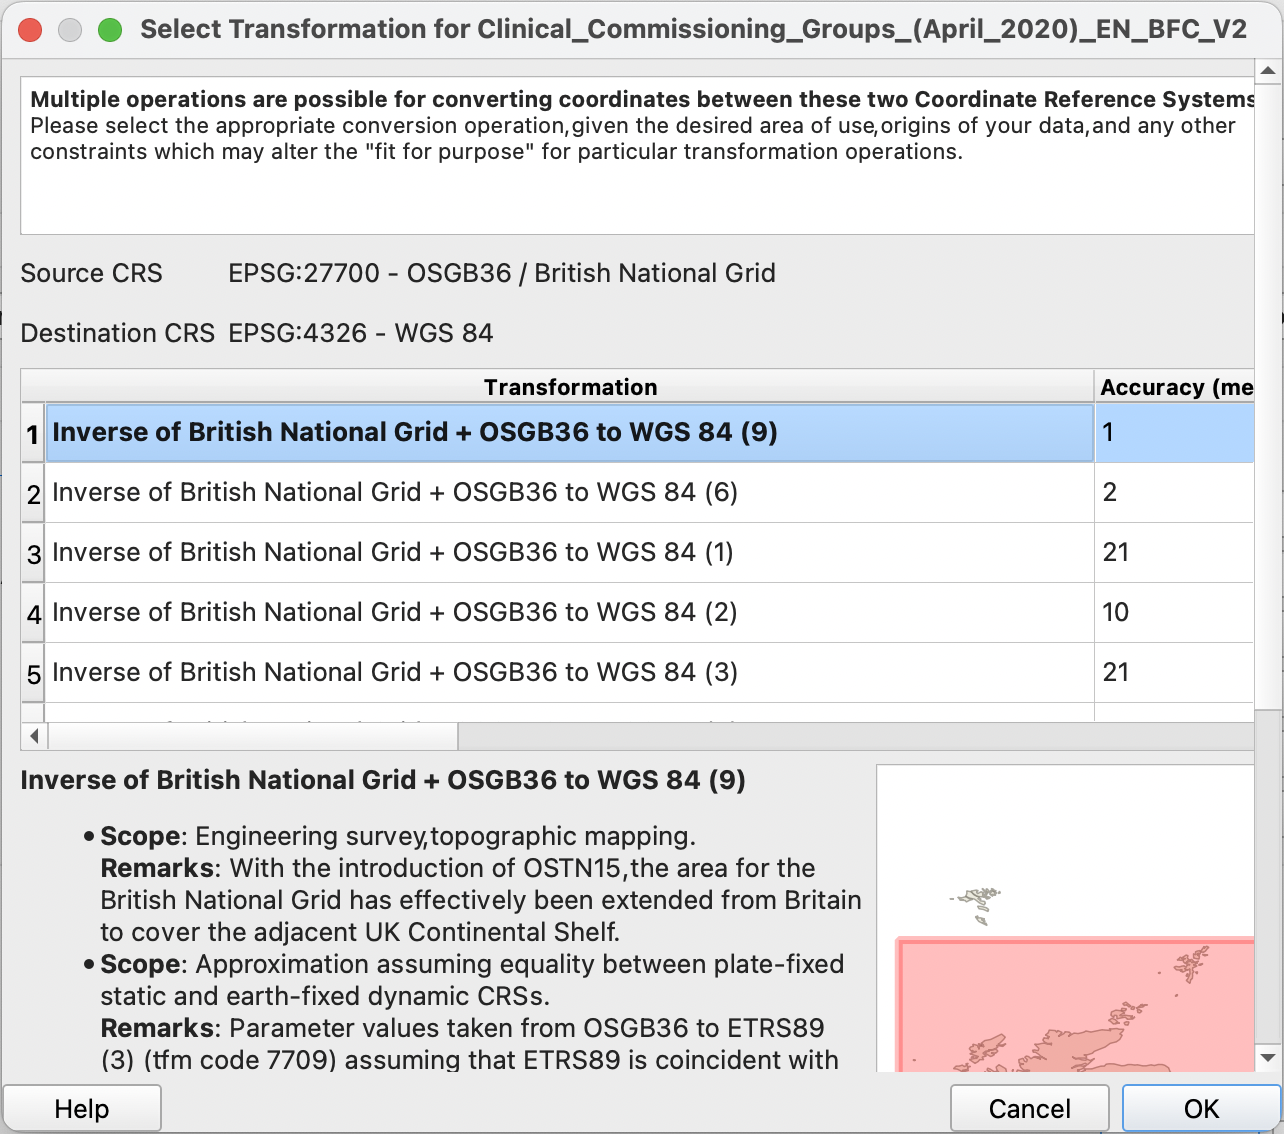
\includegraphics[width=\columnwidth]{figure/qgis/reproject.png}
    \caption{QGIS interface. A window prompt to transform the CCG shapefile's CRS into WGS-84.}
    \label{fig:reproject}
\end{figure}

\begin{figure}[h!]
    \centering
    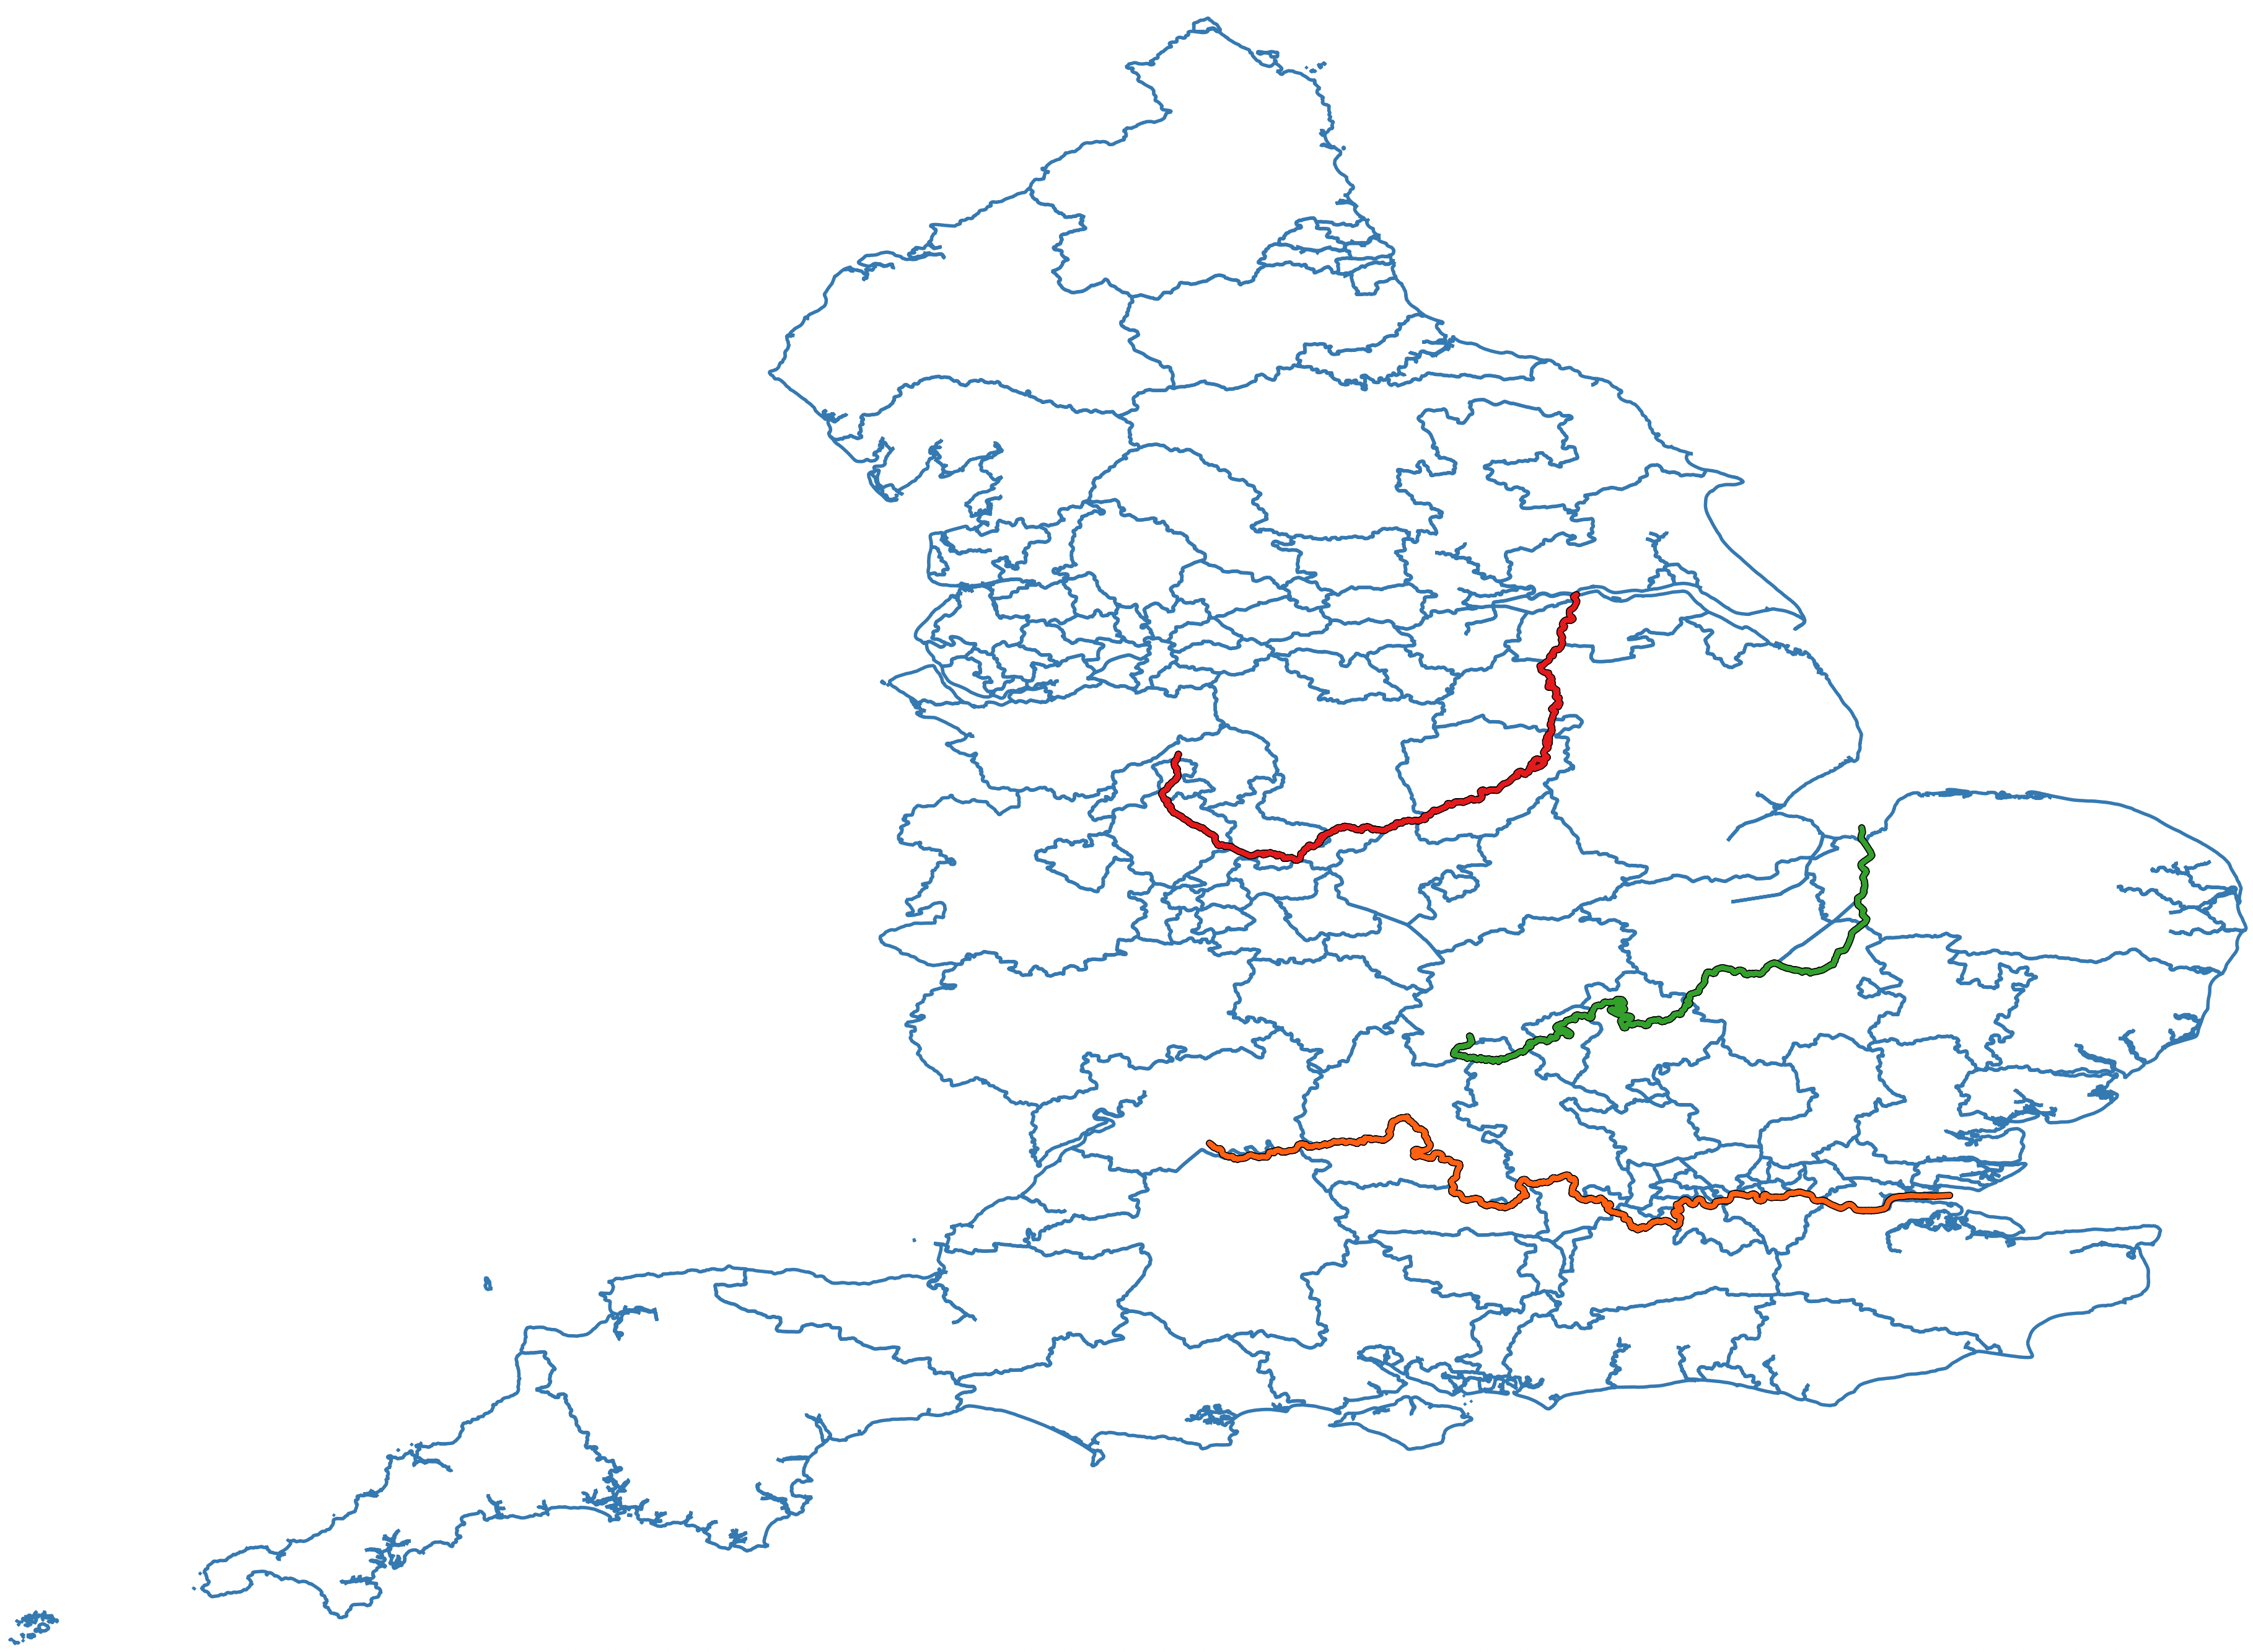
\includegraphics[width=\columnwidth]{figure/qgis/all_rivers.png}
    \caption{The reprojection result produced by \figref{fig:reproject}, which includes the River Trent (red), River Great Ouse (green), and River Thames (orange).}
    \label{fig:all_rivers}
\end{figure}
}

\section{Procedure: DerivePoint}

% \begin{noindent}

    \begin{algorithm}[h!]
        \caption{Procedure to derive a point based an edge and a distance.}\label{alg:derive corridor point}
        \textbf{Input:} \\
        $ \Edge \gets $ the edge used to derive the new point \\
        $ \Distance \gets $ the distance between $ \PointP $ and $ \EdgeStart $ \\

        \textbf{Output:} \\
        A point, $ \PointP $, that is distance $ \Distance $ away from $ \EdgeStart $. \\
    
        \textbf{Local variables:} \\
        $ \dx, \dy \gets $ the differences in $ x, y $ for $ \EdgeStart $ and $ \EdgeEnd $ \\
    
        \begin{algorithmic}[1]
            \Procedure{DerivePoint}{$ \Edge $, $ \Distance $}
                \State $ \dx \gets \EdgeStart.x - \EdgeEnd.x $
    
                \State $ \dy \gets \EdgeStart.y - \EdgeEnd.y $
    
                \State $ \PointP.x \gets \frac{\dx}{\sqrt{\dx^2 + \dy^2}} \cdot \Distance $
    
                \State $ \PointP.y \gets \frac{\dy}{\sqrt{\dx^2 + \dy^2}} \cdot \Distance $
    
            \State \Return{$ \PointP $}
    
            \EndProcedure
    
        \end{algorithmic}
    \end{algorithm}
    
%\end{noindent}

\section{Procedure: DeriveParallelEdge}

% \begin{noindent}

\begin{algorithm}[h!]
    \caption{Procedure to derive an edge, $ \EdgeParallel $, that is parallel to $ \Edge $ with a distance of $ \Distance $.}\label{alg:derive corridor edge}

    \textbf{Input:} \\
    $ \Edge \gets $ the edge used to derive the parallel edge $ \EdgeParallel $ \\
    $ \Distance \gets $ the shortest distance between $ \Edge $ and $ \EdgeParallel $ \\

    \textbf{Output:} \\
    An edge, $ \EdgeParallel $, that is parallel to $ \Edge $ with a distance of $ \Distance $. \\

    \textbf{Local variables:} \\
    $ \dx, \dy \gets $ the differences in $ x, y $ for $ \EdgeStart $ and $ \EdgeEnd $ \\
    $ \Scale \gets $ the scale of $ \frac{\Distance}{\sqrt{\dx^2 + \dy^2}} $ \\

    \begin{algorithmic}[1]
        \Procedure{DeriveParallelEdge}{$ \Edge $, $ \Distance $}
            \State $ \dx \gets \EdgeStart.x - \EdgeEnd.x $

            \State $ \dy \gets \EdgeStart.y - \EdgeEnd.y $

            \State $ \Scale \gets \frac{\Distance}{\sqrt{\dx^2 + \dy^2}} $

            \State $ \EdgeParallel.start.x \gets \Scale \cdot -\dy + \EdgeStart.x $

            \State $ \EdgeParallel.start.y \gets \Scale \cdot \dx + \EdgeStart.y $

            \State $ \EdgeParallel.end.x \gets \Scale \cdot -\dy + \EdgeEnd.x $

            \State $ \EdgeParallel.end.y \gets \Scale \cdot \dx + \EdgeEnd.y $

        \State \Return{$ \EdgeParallel $}

        \EndProcedure

    \end{algorithmic}
\end{algorithm}

%\end{noindent}